I% Chapter Template

\chapter{Performance} % Main chapter title

\label{Performance} % Change X to a consecutive number; for referencing this chapter elsewhere, use \ref{ChapterX}

\lhead{Performance. \emph{Performance in practice and Benchmarks}} % Change X to a consecutive number; this is for the header on each page - perhaps a shortened title


%----------------------------------------------------------------------------------------
%	SECTION In practice: Running on JVM
%----------------------------------------------------------------------------------------
\section{In practice: Running on JVM}
\label{InPractice}

In practice, Scala compiles to Java bytecode and executes on a JVM, where we take the Java SE HotSpot as a reference. This imposes additional characteristics of performance that can't be evaluated on the algorithmic level alone.

% code interpreted vs compiled
The JVM use \emph{just in time} (or JIT) compilation of code to take advantage of knowledge about how the code is used at runtime. At first it runs on interpreter mode, it consists of interpreting the bytecode and collecting statistics on the codes execution. Eventually it will compile the code to make it faster using several optimisations and heuristics. The code of the vectors tries to gains performance by aligning with those heuristics and hence taking advantage of the JVM optimizations.

% GC and memory allocations
One of the components of the JVM that will be affected by vectors is the garbage collector. The vector tends to create a large amount of \texttt{Arrays} during transformations, of which many are only necessary for a short time. Those objects will use up memory and possibly degrade performance of future allocations, until the next GC. Having all these unused object will also contribute in an increase in the frequency of GC executions. For that reason the code is optimised to avoid excessive creation of intermediary objects.

% memory access and caches
% system arraycopy primitive
When running on some machine we have several memory cashes helping with performance. The vector tries to align to the underlying cache model to improve performance. The size of the arrays is chosen to take advantage of cache lines while they are copied and traversed. This makes the behaviour of node copies look more as a constant time operation. Further more when copying arrays the \texttt{System.arraycopy} primitive is used. This way, the critical operation that is executed on each update will use the lowest level implementation available for the JVM. This could potentially go down to efficient host machines code when compiled.

%-----------------------------------
%	SUBSECTION Cost of Abstraction
%-----------------------------------
\subsection{Cost of Abstraction and JIT Inline}
% cost of function invokation
One of the optimizations that the JVM provides is function call elimination (abstraction elimination) based on a set of heuristics. This is equivalent to the functions optimisation in section \ref{sec:Abstractions} but done on another level of the pipeline. Critical parts of the code are written with careful detail to match the heuristics of the JVM.

% code compiled (inlined if hot)
% aim to make all critical methods 35< bytes
The optimisation works as follows: the code is run in interpretation mode first while keeping track of statistics on which parts of the code are executed and how many times. When the code is eventually compiled, function calls that are deemed \emph{hot} are inlined. The heuristic favours inline when the function has less than 35 bytes. 

We use this knowledge of the heuristic in two ways. The first is to avoid inlining everything, if the function is small and there is no other optimisation that can be done if inline manual, the code is kept as a function. The second is to inline the methods of the vector API into the clients code. When implementing functions with less than 35 bytes, performance was tested and cross referenced with the VMs inlining diagnostic\footnote{The JVMs \texttt{"-XX:+UnlockDiagnosticVMOptions -XX:+PrintInlining"} flag was used to track the inlining.}. The code was inspected using \texttt{javap -c}, which gives the sizes of the function and helped identifying some optimisation possibilities.

%----------------------------------------------------------------------------------------
%	SECTION Scalameter
%----------------------------------------------------------------------------------------
\clearpage
\section{Measuring performance}
% Scalameter
ScalaMeter framework\cite{scalameter} is used to measure performance of operations on different implementations of vector. This framework was used to spot identify performance improvements or regressions during the development process. 

% warmup to compile code and reduce jitter (JIT, GC)
To have reproducible results with low error margins, ScalaMeter was configured on a per benchmark basis\footnote{The JVM \texttt{-XX:+PrintCompilation} flag vas used to help identifying the ideal configuration.}. Each test is run on 32 different JVM instances to average out badly allocated VMs. On each JVM 32 measurements are taken, while using outlier elimination to remove benchmark runs that where exceptionally different. This could happen if one particular run has a garbage collection, JIT compilation of code or OS executing something else. Before the benchmark runs the JVM is warmed up by running some times the benchmark without taking measurements. During these first execution the VM will be loading classes, taking some statistic on the code and then eventually compiling it.

% types of vectors
There are two main axis of performance comparisons. The first is between the RB-Vector and a perfectly balanced RRB-Tree where the aim is to have an equivalent performance, even if the RRB-Vector have an inherent additional overhead. The second axis is the one that shows the effects of unbalanced nodes on RRB-Tree. For this we compare the same perfect balanced vector with one that is the result of one concatenation of two vectors and with an extremely unbalanced vector. The later vector is generated by concatenating random\footnote{Pseudo random generator where used to be able to reproduce the same ones each time.} small vectors together. The amount of unbalanced nodes is in part affected by the size of the vector. Other axes are discussed in the next section.

%----------------------------------------------------------------------------------------
%	SECTION Generators
%----------------------------------------------------------------------------------------
\clearpage
\section{Implementation Generators}
Until now only one implementation of the RRB-Vector\footnote{Located in the \texttt{scala.collection.immutable.rrbvector} package on GitHub} that is compared against the RB-Vector. But in fact to compare performance on different characteristics like block sizes and concatenation algorithm variant concrete implementations where generated using Scala reflection. Other characteristics involve a complete structure assertion while testing and benchmarks generation. For each combination of characteristics there is a concrete artefact: class implementation, tests and benchmarks.

Code is generated by combining AST using Quasiquotes with some domain specific optimizations. The optimizations are the same that where applied manually on the main implementation of the RRB-Vector. The resulting code is equivalent, except that it lacks formatting. The name of the artefact is used to identify the different characteristics\footnote{All generated artefacts are in the \texttt{scala.collection.immutable.generated.rrbvector} package on GitHub}.

% block sizes
The block sizes used where 32, 64, 128 and 256. 
The main aim is the differences in performances of the operations and identify sizes for which permanence degrades due to loss of cache locality. 
This is the only number in the name of the artefact.

% concat implementation
Both version of the RRB-Vector are to generate vectors. 
This done mostly to compare the performances of other operation on vector that got unbalanced using concatenation. 
\texttt{Complete} (or \texttt{c} in the name of the artefact) is used to name identify the version that rebalances completely the subtree. 
The other one is named \texttt{Quick} or \texttt{q} in the name of the artefact.

% testing
For testing purposes, for each implementation there is a second one generated with heavy assertions on the whole structure of the vector on most methods (see \ref{InvariantAssertions}). 
Concrete benchmarks are also generated at the same time.

Generating this code was the only reasonable way to implement this huge amount of classes while implementing new features on them. 
Changes that would otherwise had to be propagated by hand on each one. 
This also help to find and fix bugs, because a bug has a higher probability of affecting at leas one of the artefact and a fixed bug fixes it on all of them.

%----------------------------------------------------------------------------------------
%	SECTION Benchmarks
%----------------------------------------------------------------------------------------
\clearpage
\section{Benchmarks}
% reiterate the the different benchmark types 
%% differences between implementation (vector vs rrbvector)
%% differences between unbalances
%% differences between block sizes
%% differences between concatenation rebalancing method
% benchmarks on core operations
Performance benchmarks aim to compare the performance of all core operations of the vectors RRB-Trees. These operations are: \texttt{apply}, \texttt{concatenate}, \texttt{append}, \texttt{prepend}, \texttt{take}, \texttt{drop}. The performance of specialized operations for the iterators, builder and the parallel vector where also benchmarked. Additionally, the memory footprint of different vectors was checked.

The axis of comparisons are: 
\begin{itemize}
	\item Size of the vector. Split into ranges that correspond to vectors of the same height, when perfectly balanced.
	\item \texttt{Vector} against completely balanced \texttt{RRBVector}
	\item Differently balanced \texttt{RRBVector}s: perfectly balanced, unbalanced (by one concatenation) and extremely unbalanced. This is ignored on vector of depth lesser than 3 because there all those vectors end up being perfectly balanced.
	\item Different block sizes: 32 (original), 64, 128 and 256.
	\item Different implementation of the rebalancing in \texttt{concatenate}: Complete rebalance and Quick rebalance
	\item Thread pool size for parallel vectors.
\end{itemize}

% machine description
For the results of this sections, All benchmarks where executed on a Java HotSpot(TM) 64-Bit Server VM on a machine with an Intel(R) Core(TM) i7-4770 CPU @ 3.40GHz with 32GiB on RAM. Each benchmarking VM instance was setup with 16GiB of heap memory. 

%-----------------------------------
%	SUBSECTION Apply
%-----------------------------------
\subsection{Apply}
% describe the benchmark function
The \texttt{apply} benchmarks aim to see the amortised access time of elements. Amortising the displays optimisation and memory caches. For this, each benchmark invokes the \texttt{apply} operation $10k$ times on different elements. 

There are two variants: the first variant access the elements sequentially and the second one chooses each time a random index. The first one is supposed to have better performance because the array that are access tend to be in cache. The computations of the next index is also a bit more complex on the second one, but mostly irrelevant compared with the cache misses of all the arrays on a branch.

% compare expectation with results
% explain the upper bound
The benchmark results for the sequential access in figures \ref{ApplyBenchmarks2} and \ref{ApplyBenchmarks3} show that if the RRB-Vector is balanced or just sightly unbalanced will be faster than the RB-Vector. But when it gets extremely unbalanced the performance can drop by around 0.5X which is proportional to the increase of arrays that must be accessed (two per node).

\begin{figure}[h!]
  \centering
  \includegraphics[width=\textwidth]{Benchmarks/Apply_2.pdf}
  \caption{Time to execute 10k apply operations on sequential indices on vectors of height 2.}
   \label{ApplyBenchmarks2}
\end{figure}

The performance improvements where achieved by analysing the sizes of the functions involved, there inlining and which parts of the code is used in each case. The aim was to improve performance of unbalanced vectors, that is why in some cases the slightly unbalanced vector is the faster.

\begin{figure}[h!]
  \centering
  \includegraphics[width=\textwidth]{Benchmarks/Apply_3.pdf}
  \caption{Time to execute 10k apply operations on sequential indices on vectors of height 3.}
   \label{ApplyBenchmarks3}
\end{figure}

\FloatBarrier

Figure \ref{ApplyRandomBenchmarks} show the results for random indices. It can be observed that the behaviour of the curve is quite similar, but the sequential one is around 2X faster due to memory locality.

\begin{figure}[h!]
  \centering
  \includegraphics[width=\textwidth]{Benchmarks/Apply_random_3.pdf}
  \caption{Time to execute 10k apply operations on random indices on vectors of height 3.}
  \label{ApplyRandomBenchmarks}
\end{figure}

\FloatBarrier

Finally, the figures \ref{ApplyBlocksBenchmarks} show what would happen if the block sizes changed or if the rebalance algorithm is changed. Note that in the cases for blocks of 128 and 256 the complete rebalance is actually creating completely balanced vectors. It can be observed that the quick rebalance is nocive to the performance of the apply method. Increasing the sizes of the arrays will improve the performance of the apply method.

\begin{figure}[h!]
  \centering
  \includegraphics[width=0.49\textwidth]{Benchmarks/Apply_blocks_32.pdf}
  \includegraphics[width=0.49\textwidth]{Benchmarks/Apply_blocks_64.pdf}
  \includegraphics[width=0.49\textwidth]{Benchmarks/Apply_blocks_128.pdf}
  \includegraphics[width=0.49\textwidth]{Benchmarks/Apply_blocks_256.pdf}
   \caption{Time to execute 10k apply operations on sequential indices. Comparing performances for different block sizes and different implementation of the concatenation inner branch rebalancing (Complete/Quick).}
  \label{ApplyBlocksBenchmarks}
\end{figure}

\FloatBarrier

%-----------------------------------
%	SUBSECTION Concatenation
%-----------------------------------
\subsection{Concatenation}
% describe the benchmark function
The \texttt{concatenation} benchmarks aim to show the benefit of having the logarithmic concatenation algorithm against the linear version. The benchmarks concatenate two vectors of the same type and balance characteristics. As such these benchmarks have two axis representing the sizes of the LHS and RHS vector in the operation.


% compare expectation with results
% explain the upper bound
% explain apparently incoherent results

Figure \ref{ConcatBenchmarks} shows how the concatenation time for RB-Vectors is linear on the size of the resulting vector. Below that, the three surfaces that represent the RRB-Vector concatenation are effectively constant time (or $log_{32}(n)$). The performance difference between the differently balanced RRB-Vectors is negligible in relation to the difference with RB-Vector. 

\begin{figure}[h!]
  \centering
  \includegraphics[width=\textwidth]{Benchmarks/Concat.png}
  \caption{Execution time for a concatenation operation on two vectors. In theory (and in practice) Vector concatenation is $O(left + right)$ and the rrbVector concatenation operation is $O(log_{32}(left + right))$.}
   \label{ConcatBenchmarks}
\end{figure}

In the case of concatenation, being balanced or not does not impose performance improvements or degradations. Performance will be determined by the number elements in the branches that get merged and their alignment.

The benchmark for the Quick rebalancing version where not included here because the implementation for that one is suboptimal and the comparison would not be fair. The main purpose of that version is to show the differences it would cause on other operation. The current version of the Quick rebalancing can achieve 2X performance benefit, but it could gain a lot form the same optimizations that were used on the Complete rebalancing.

\FloatBarrier

%-----------------------------------
%	SUBSECTION Append
%-----------------------------------
\subsection{Append}
% describe the benchmark function
The \texttt{append} benchmarks aim to see the amortised time taken to appending elements. With the transient states, the branch updates are amortized over leaf updates. For this, each benchmark appends 256 elements on a vector. This way there is at least one branch update for each benchmark, 8 if the block size is 32.

\begin{figure}[h!]
  \centering
  \includegraphics[width=\textwidth]{Benchmarks/Append_2.pdf}
  \caption{Time to execute 256 append operations on vectors of height 2. This shows the amortized cost of the append operation.}
  \label{Append2Benchmarks}
\end{figure}

% compare expectation with results
% explain the upper bound
% explain apparently incoherent results
The figures \ref{Append2Benchmarks} and \ref{Append3Benchmarks} show that if the RRB-Vectors are balanced or just slightly unbalanced the execution time is equivalent to the one for RB-Vectors. But, if it gets extremely unbalanced the performance can fall to by 0.6X. In figure \ref{Append2Benchmarks} it is possible to see that after 768 the performance does a step upward, this correspond to the addition of a level in the tree.

\begin{figure}[h!]
  \centering
  \includegraphics[width=\textwidth]{Benchmarks/Append_3.pdf}
  \caption{Time to execute 256 append operations on vectors of height 3. This shows the amortized cost of the append operation.}
   \label{Append3Benchmarks}
\end{figure}

\FloatBarrier

Finally, the figures \ref{AppendBlocksBenchmarks} show what would happen if the block sizes changed or if the rebalance algorithm is changed. Note that in the cases for blocks of 128 and 256 the complete rebalance is actually creating completely balanced vectors (from $16384$ down in the case of 128). It can be observed that the quick rebalance is nocive to the performance of the append method. Increasing the sizes of the arrays will decrease the performance for balanced trees, but can potentially reduce the amount of unbalanced nodes in the extremely unbalanced trees.

\begin{figure}[h!]
  \centering
  \includegraphics[width=0.49\textwidth]{Benchmarks/Append_blocks_32.pdf}
  \includegraphics[width=0.49\textwidth]{Benchmarks/Append_blocks_64.pdf}
  \includegraphics[width=0.49\textwidth]{Benchmarks/Append_blocks_128.pdf}
  \includegraphics[width=0.49\textwidth]{Benchmarks/Append_blocks_256.pdf}
  \caption{Time to execute 256 append operations. This shows the amortized cost of the append operation. Comparing performances for different block sizes and different implementation of the concatenation inner branch rebalancing (Complete/Quick).}
  \label{AppendBlocksBenchmarks}
\end{figure}



\FloatBarrier

%-----------------------------------
%	SUBSECTION Prepend
%-----------------------------------
\subsection{Prepend}
% describe the benchmark function
The \texttt{prepend} benchmarks aim to see the amortised time taken to prepending elements. With the transient states, the branch updates are amortized over leaf updates. For this, each benchmark appends 256 elements on a vector. This way there is at least one branch update for each benchmark, 8 if the block size is 32.

% compare expectation with results
% explain the upper bound
% explain apparently incoherent results

\begin{figure}[h!]
  \centering
  \includegraphics[width=\textwidth]{Benchmarks/Prepend_2.pdf}
  \caption{Time to execute 256 prepend operations on vectors of height 2. This shows the amortized cost of the prepend operation.}
  \label{Prepend2Benchmarks}
\end{figure}

The figures \ref{Prepend2Benchmarks} and \ref{Prepend3Benchmarks} show that the prepend operation on a balanced RRB-Vector is a bit slower. This is because prepending on this kind of vector requires the creation or update of an unbalanced node. But, this is a a case where the unbalanced vectors end up being more performant. This is because on these vectors there it is possible to find space to perpend elements on the left of the tree. In figure \ref{Prepend2Benchmarks} it is possible to see that after 768 the performance does a step upward, this correspond to the addition of a level in the tree.

\begin{figure}[h!]
  \centering
  \includegraphics[width=\textwidth]{Benchmarks/Prepend_3.pdf}
  \caption{Time to execute 256 prepend operations on vectors of height 3. This shows the amortized cost of the prepend operation.}
  \label{Prepend3Benchmarks}
\end{figure}

\FloatBarrier

Finally, the figures \ref{PrependBlocksBenchmarks} show what would happen if the block sizes changed or if the rebalance algorithm is changed. Note that with 128 and 256 there are some performance degradation. They probably reflect the limit in cacheline locality where the node updates become linear again due to memory accesses and updates. The performance for blocks of size 32 and 64 are quite similar, but it is more stable for 64 because it needs a lesser number of branch updates.

\begin{figure}[h!]
  \centering
  \includegraphics[width=0.49\textwidth]{Benchmarks/Prepend_blocks_32.pdf}
  \includegraphics[width=0.49\textwidth]{Benchmarks/Prepend_blocks_64.pdf}
  \includegraphics[width=0.49\textwidth]{Benchmarks/Prepend_blocks_128.pdf}
  \includegraphics[width=0.49\textwidth]{Benchmarks/Prepend_blocks_256.pdf}
  \caption{Time to execute 256 prepend operations. This shows the amortized cost of the append operation. Comparing performances for different block sizes and different implementation of the concatenation inner branch rebalancing (Complete/Quick).}
  \label{PrependBlocksBenchmarks}
\end{figure}

\FloatBarrier

%-----------------------------------
%	SUBSECTION Splits
%-----------------------------------
\subsection{Splits}
% describe the benchmark function
% compare expectation with results
% explain the upper bound
% explain apparently incoherent results
\color{red} TODO \color{black}

\begin{figure}[h!]
  \centering
  \includegraphics[width=\textwidth]{Benchmarks/Split_take_3.pdf}
  \label{TakeBenchmarks}
  \caption{Execution time of take.}
\end{figure}


\begin{figure}[h!]
  \centering
  \includegraphics[width=\textwidth]{Benchmarks/Split_drop_3.pdf}
  \label{DropBenchmarks}
  \caption{Execution time of drop.}
\end{figure}


\FloatBarrier

%-----------------------------------
%	SUBSECTION Iterator
%-----------------------------------
\subsection{Iterator}
% describe the benchmark function
The iteration benchmarks aim to see the performance of traversing the whole vector using an iterator. Linear behaviour is expected from these benchmarks.

\begin{figure}[h!]
  \centering
  \includegraphics[width=\textwidth]{Benchmarks/Iteration_3.pdf}
  \caption{Excecution time to iterate through all the elements of the vector.}
  \label{Iteration2Benchmarks}
\end{figure}

% compare expectation with results
% explain the upper bound
% explain apparently incoherent results: iteration of sightly unbalanced vector is faster
Figures \ref{Iteration2Benchmarks} and \ref{Iteration3Benchmarks} show that for balanced RRB-Vectors the performances is identical. For slightly unbalanced once there is an increase in performance that seams to come from JIT optimizations of the code. In that case the code that is used to change branches uses fewer lines of code in each function (some are never access at runtime), it could be possible that the optimiser is using this to improve the performance\footnote{Further analysis on this situation should be done in the future.}. 

\begin{figure}[h!]
  \centering
  \includegraphics[width=\textwidth]{Benchmarks/Iteration_4.pdf}
  \caption{Excecution time to iterate through all the elements of the vector.}
  \label{Iteration3Benchmarks}
\end{figure}

When the vectors become extremely unbalanced, the performance degenerates by a factor proportional to the height of the vector. Because it changes from one balanced subtree to the next one from the root. It should be possible, by keeping more state in the iterator, to improve the performance to go from one balanced subtree to the next. But this would increase the initialisation time and might affect smaller vectors.

\FloatBarrier

Finally, the figures \ref{IterationBlocksBenchmarks} show what would happen if the block sizes changed or if the rebalance algorithm is changed. In general the quick rebalancing is usually worst than complete rebalancing for the iterator. The block sizes do not change much the performance of the iterator. This is a great result because it means that the overhead of traversing the tree is insignificant when traversing the vector, the cost is in the traversal of the leafs.

\begin{figure}[h!]
  \centering
  \includegraphics[width=0.49\textwidth]{Benchmarks/Iteration_blocks_32.pdf}
  \includegraphics[width=0.49\textwidth]{Benchmarks/Iteration_blocks_64.pdf}
  \includegraphics[width=0.49\textwidth]{Benchmarks/Iteration_blocks_128.pdf}
  \includegraphics[width=0.49\textwidth]{Benchmarks/Iteration_blocks_256.pdf}
  \caption{Excecution time to iterate through all the elements of the vector. Comparing performances for different block sizes and different implementation of the concatenation inner branch rebalancing (Complete/Quick).}
  \label{IterationBlocksBenchmarks}
\end{figure}

\FloatBarrier

%-----------------------------------
%	SUBSECTION Builder
%-----------------------------------
\subsection{Builder}
% describe the benchmark function
The builder benchmarks aim to show the time it takes to build a vector of some size by appending elements. The performance of this is expected to be linear. Note that all vectors that are generated will be completely balanced.

% compare expectation with results

\begin{figure}[h!]
  \centering
  \includegraphics[width=\textwidth]{Benchmarks/Builder_3.pdf}
  \caption{Execution time to build a vector of a given size.}
    \label{Builder3Benchmarks}
\end{figure}

Figures \ref{Builder3Benchmarks} and \ref{Builder4Benchmarks} show that the RB and RRB vector builder have the same results. This is not surprising, because the have the same code for appending elements, except for a small detail. The RRB Vector allocates arrays with one additional slot for all branch nodes.

\begin{figure}[h!]
  \centering
  \includegraphics[width=\textwidth]{Benchmarks/Builder_4.pdf}
  \caption{Execution time to build a vector of a given size.}
   \label{Builder4Benchmarks}
\end{figure}

\FloatBarrier

Increasing the sizes of the blocks will reduce the amounts of blocks that need to be allocated during the building. Larger block will also take slightly longer to allocate. Figure \ref{BuilderBlocksBenchmarks} shows that the difference is not really big, but with a sweet spot on blocks of size 64 for builders.

\begin{figure}[h!]
  \centering
  \includegraphics[width=\textwidth]{Benchmarks/Builder_blocks.pdf}
  \caption{Execution time to build a vector of a given size. Comparing performances for different block sizes.}
  \label{BuilderBlocksBenchmarks}
\end{figure}

\FloatBarrier

%-----------------------------------
%	SUBSECTION Parallel split-combine
%-----------------------------------
\subsection{Parallel split-combine}
% describe the benchmark function
The aim of the parallel benchmarks is to show the overhead of the parallel framework. Specifically, the time spent in splitting and combining the vectors during parallel execution. For this the benchmarks execute a \texttt{map} on the identity function\footnote{The function that simply returns the element passed as parameter.}. This operation is done on the standard sequential version of the vector and on the parallel one.

% compare expectation with results
% explain the upper bound
% explain apparently incoherent results
In figure \ref{ParallelBenchmarks} it can be seen that the base sequential \texttt{map} is exactly the same for both implementation. This was expected because the \texttt{map} implementation uses an \texttt{iterator} and \texttt{builder} to compute it in both cases, which have the same performance. 

\begin{figure}[h!]
  \centering
  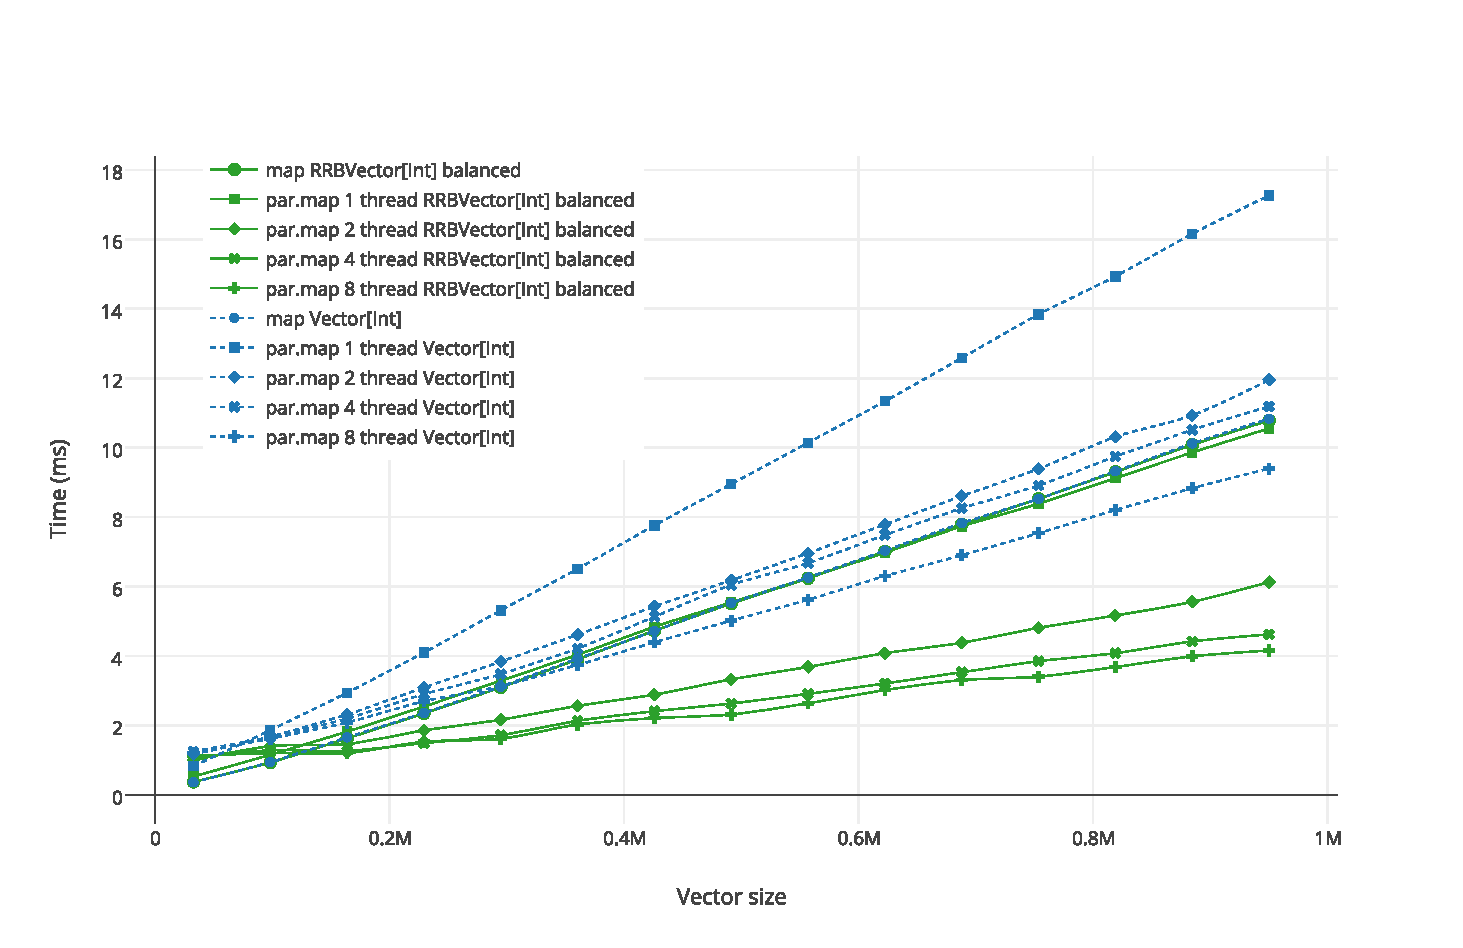
\includegraphics[width=\textwidth]{Benchmarks/Parmap_balanced.pdf}
  \caption{Benchmark on map and parallel map using the function (\textsc{x=>x}) to show the difference time used in the framework. This time represents the time spent in the splitters and combiners of the parallel collection (iterator and builder for the sequential version).}
  \label{ParallelBenchmarks}
\end{figure}

The current parallel \texttt{Vector} (that uses RB-Trees) results show that with 1, 2 and 4 threads the performance of the operation is worse. With 8 threads it becomes a little bit faster. This is what we expected, due to the lazy concatenation at the end of the combination of results. But, it show that this parallel collection is useless in practice.

When using the the RRB-Vectors parallel, the parallelism is evident. With two threads the performance improvement is of almost 2X, then it tends to go towards 2.5X. This is the type of parallelism behaviour that is expected (see Amdahl's law\cite{TODO}). Even the case on thread pool of one thread is a bit faster than the normal sequential one.

\FloatBarrier

Figure \ref{ParallelUnbalancedBenchmarks} shows how unbalanced parallel vector behave. There is a slight loss in performance when they are unbalanced. But, this operations will create a balanced vector and therefore this small overhead can be amortized over the next operations.

\begin{figure}[h!]
  \centering
  \includegraphics[width=0.49\textwidth]{Benchmarks/parmap_unbalanced_1.pdf}
  \includegraphics[width=0.49\textwidth]{Benchmarks/parmap_unbalanced_2.pdf}
  \includegraphics[width=0.49\textwidth]{Benchmarks/parmap_unbalanced_4.pdf}
  \includegraphics[width=0.49\textwidth]{Benchmarks/parmap_unbalanced_8.pdf}
  \caption{Benchmark on map and parallel map using the function (\textsc{x=>x}) to show the difference time used in the framework. This time represents the time spent in the splitters and combiners of the parallel collection.}
  \label{ParallelUnbalancedBenchmarks}
\end{figure}

\FloatBarrier

%-----------------------------------
%	SUBSECTION Memory footprint
%-----------------------------------
\subsection{Memory footprint}
% describe the benchmark function
This is not really a benchmark, it is rather the characterisation of the memory footprint of the vector that where used as input in the benchmarks. The aim of this is to show that even with the additional sizes of the unbalanced nodes and additional fields, the vectors size in memory is almost the same.

% compare expectation with results
% explain the upper bound
% explain apparently incoherent results
Figure \ref{MemoryFootprints} shows that even for an extremely unbalanced RRB-Vector the increase in size is negligible. Fact for balanced ones it is even possible to have a smaller footprint (a few bytes) caused by the truncation of the last branch. 

\begin{figure}[h!]
  \centering
  \includegraphics[width=\textwidth]{Benchmarks/Memory_3.pdf}
  \caption{Memory Footprint for different vectors.}
  \label{MemoryFootprints}
\end{figure}

\FloatBarrier

Figure \ref{MemoryBlocksFootprints} shows the amount of space that could be saved by increasing the size of the block. The difference is not significant and as such the memory footprint is not a reason to change the size of blocks.

\begin{figure}[h!]
  \centering
  \includegraphics[width=\textwidth]{Benchmarks/Memory_blocks.pdf}
  \caption{Memory Footprint for different block sizes.}
  \label{MemoryBlocksFootprints}
\end{figure}

\FloatBarrier

